\section{Gameplay}
\textit{Hyper} was designed as an \textit{open world} game.
In a game of this type, the player is not constrained to achieving a specific goal and has a large degree of freedom to explore, interact with, or modify the game environment \cite{Open-World-MW}.
In this section, we'll show the various aspects of this concept in our game.

\subsection{Terrain editing}
The player has three "terrain modifiers", represented with pickaxe symbols, at their disposal.
Using the terrain modifier, the player can edit the game's landscape by building new structures or digging in the ground.
As an example of the "creation capabilities", we show in \autoref{fig:hyper-logo} how the letters making up the game's name could be created inside the game.
\begin{figure}[!htb]
    \centering
    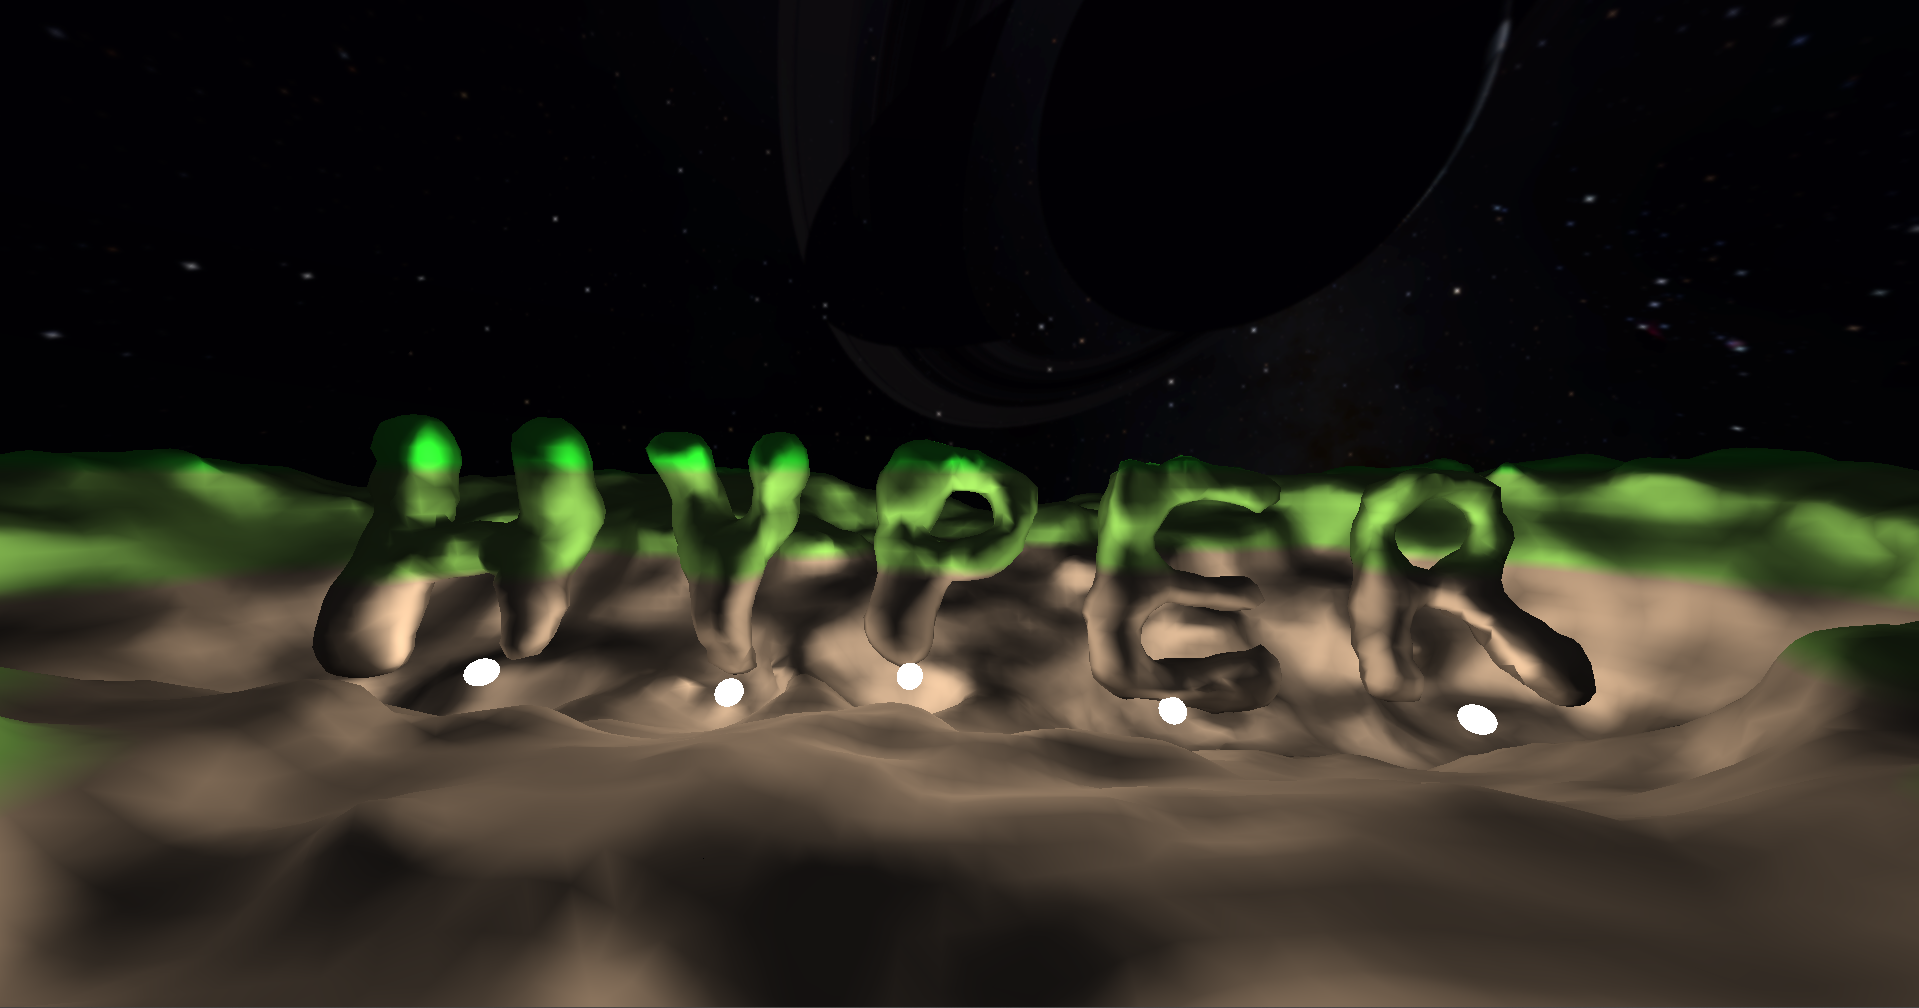
\includegraphics[width=0.8\textwidth]{chapters/results/sections/gameplay/resources/hyper-logo-night-2.png}
    \caption{The letters of the word "Hyper" created in the game}
    \label{fig:hyper-logo}
\end{figure}

As mentioned before the terrain modifiers can also be used for carving in the terrain.
To illustrate that, in \autoref{fig:tunnel-under-hill} we show a tunnel that was dug through a hill.
\begin{figure}[!htb]
    \centering
    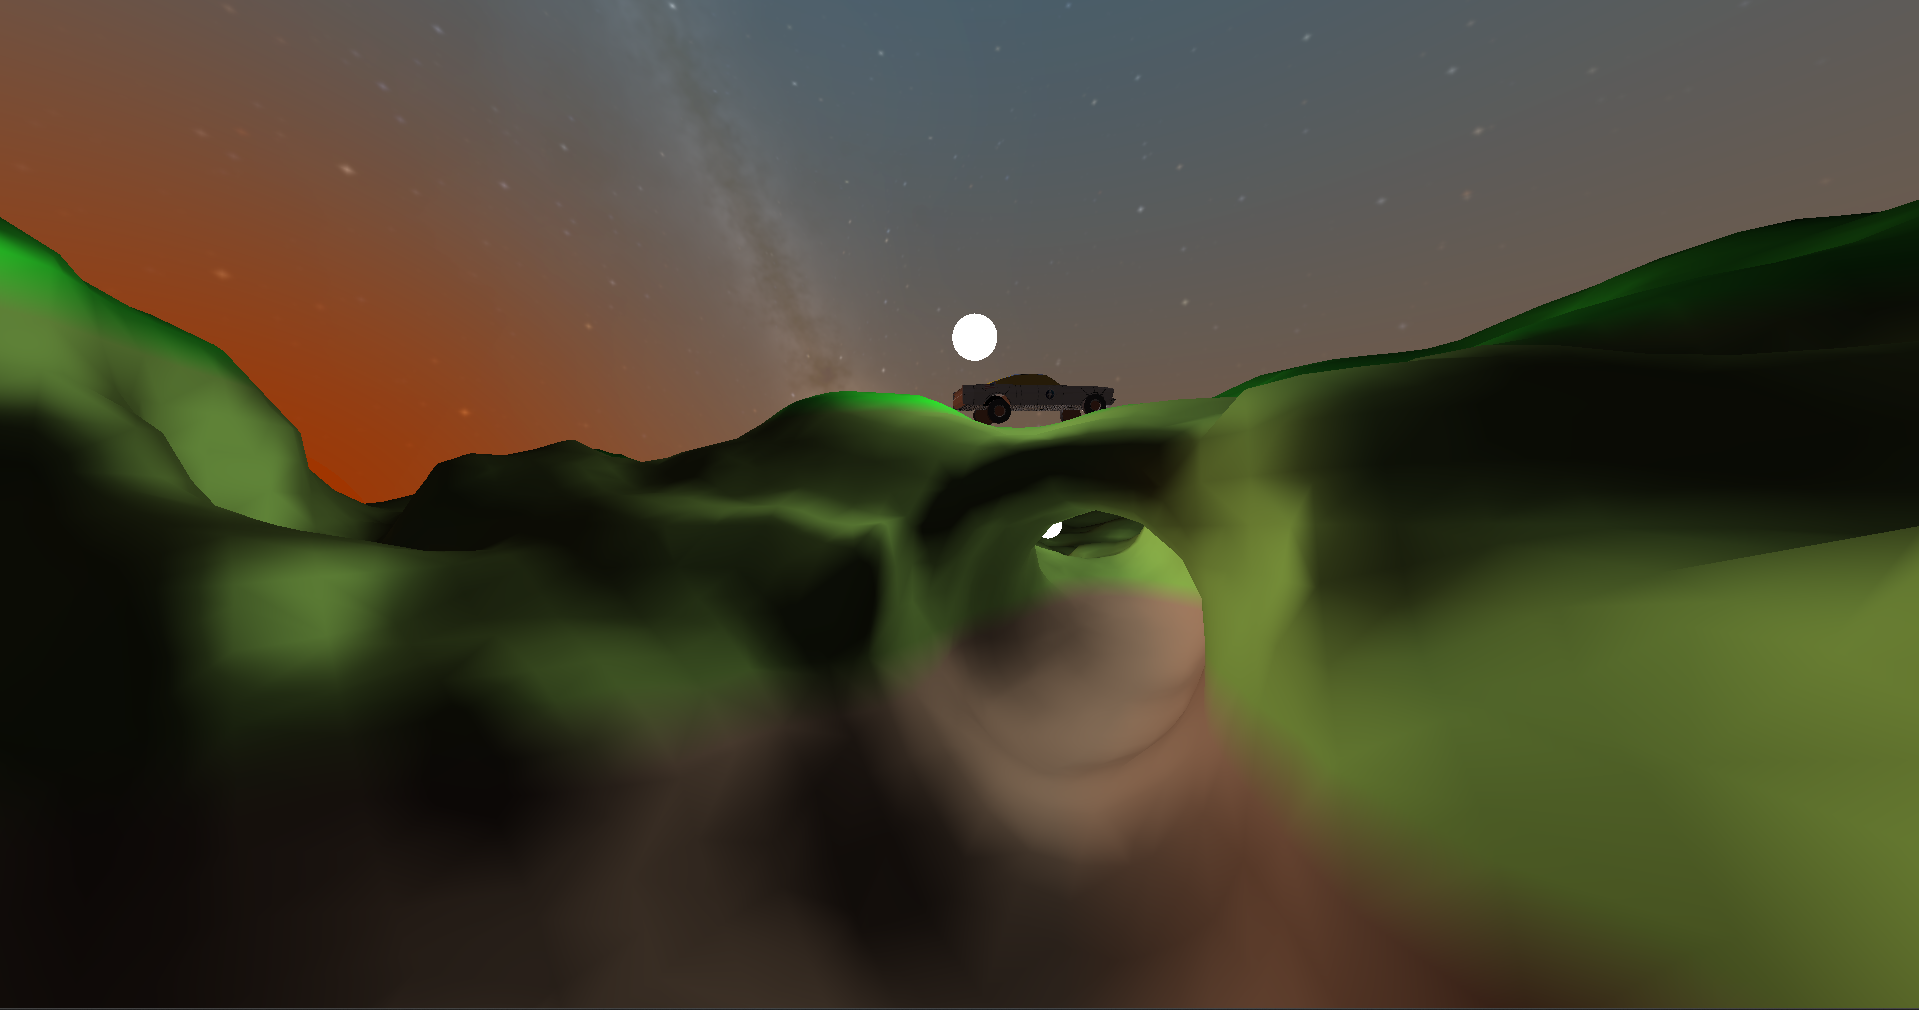
\includegraphics[width=0.8\textwidth]{chapters/results/sections/gameplay/resources/tunnel-with-car.png}
    \caption{Tunnel dug under a hill}
    \label{fig:tunnel-under-hill}
\end{figure}

\subsection{Exploring the game world}
The game starts in one of the various "landscapes" such as a desert, a forest, etc. each characterized by different terrain generation parameters and colors.

To make exploring the game world easier, the player can get into a car that moves considerably faster than the player.
\autoref{fig:car-in-hyperbolic} shows the car driving in hyperbolic space.
\begin{figure}[!htb]
    \centering
    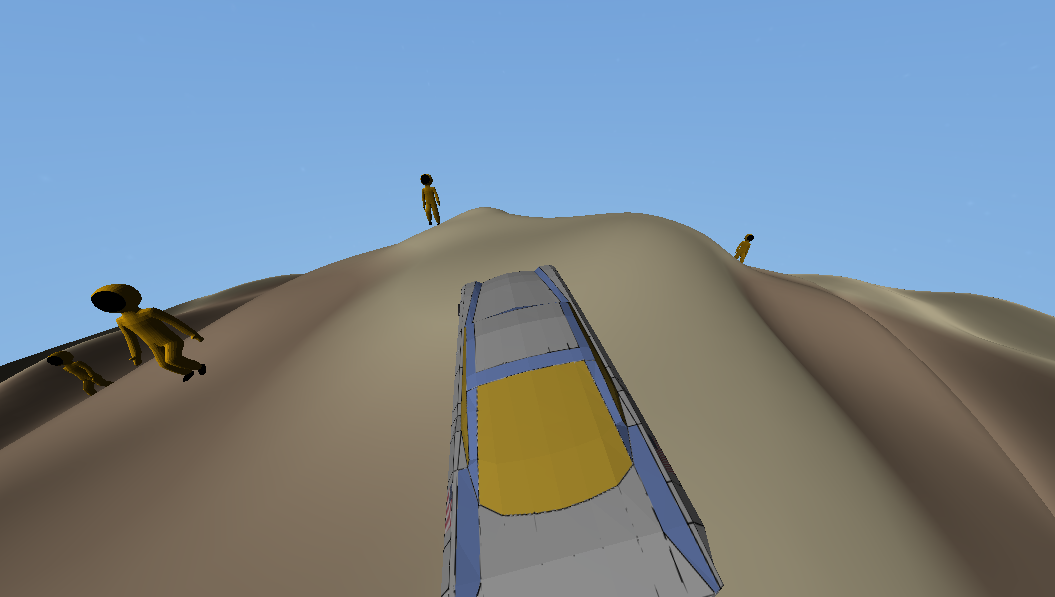
\includegraphics[width=0.8\textwidth]{chapters/results/sections/gameplay/resources/car-in-hyperbolic.png}
    \caption{Riding a car in hyperbolic space}
    \label{fig:car-in-hyperbolic}
\end{figure}
Even though the car is much faster than the player it can roll over when traversing a particularly bumpy terrain.
For this reason, we included an option to flip the car back on its wheels when that happens.
\subsection{Interacting with the world's inhabitants}
To make the world more interactive we decided to populate it with NPCs also called bots.
Bots can be either hostile toward the player or neutral.
Hostile bots shoot projectiles and walk toward the player once they get into the player's proximity.
A group of bots shooting projectiles at the player in spherical space is shown in \autoref{fig:firing-squad}.
\begin{figure}[!htb]
    \centering
    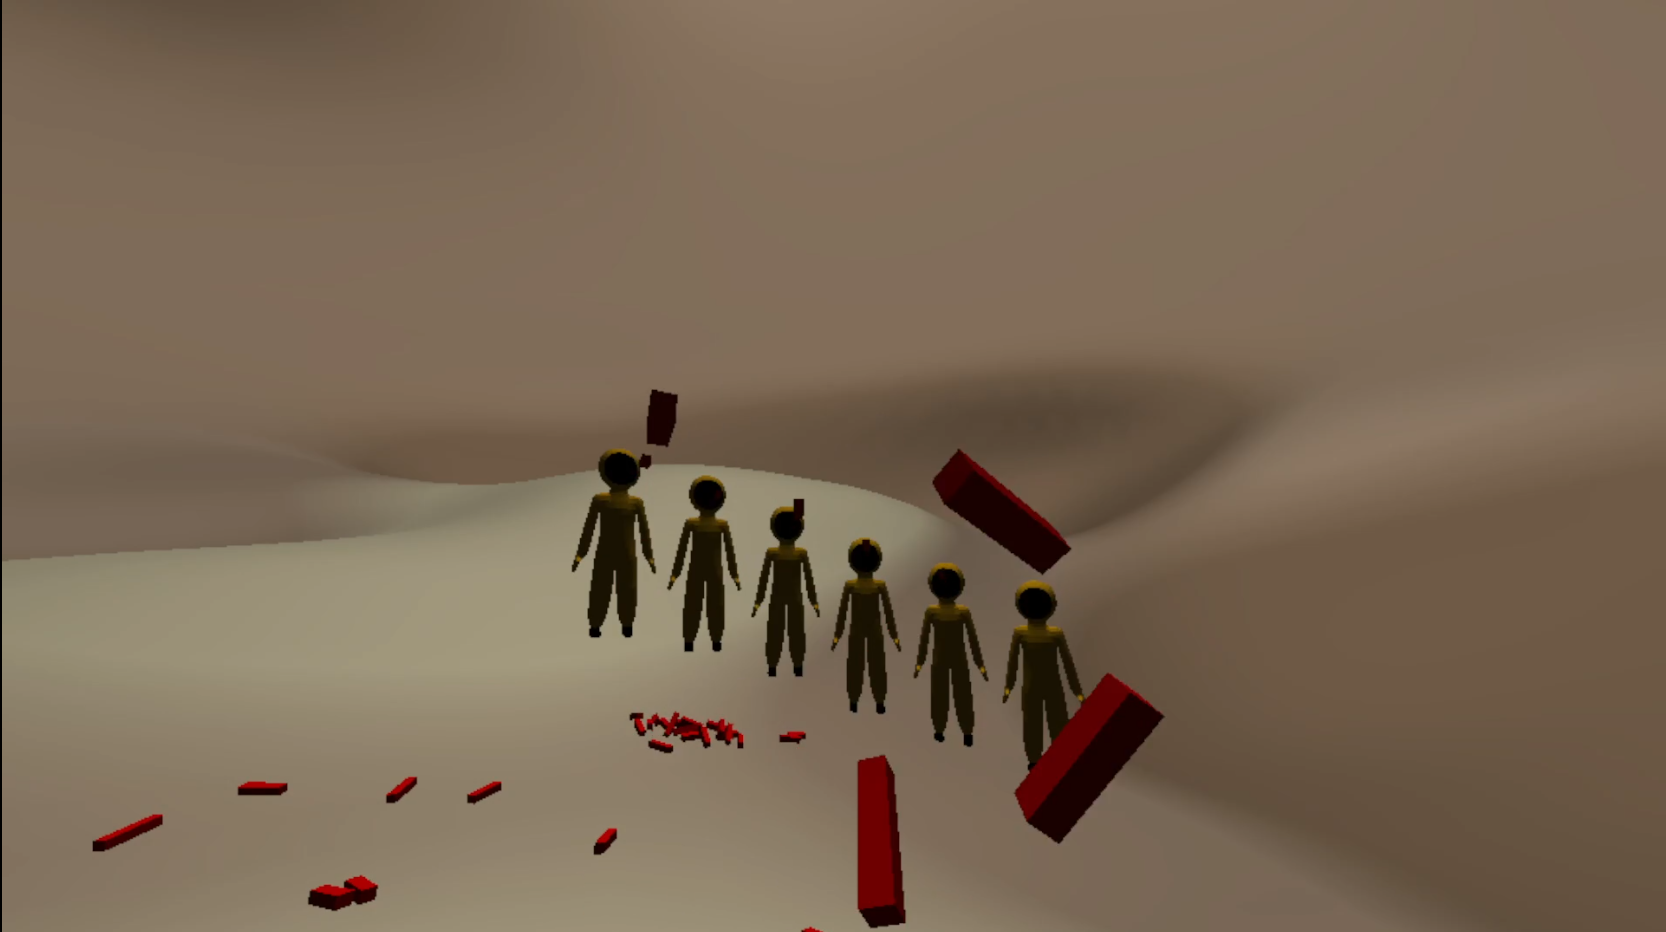
\includegraphics[width=0.8\textwidth]{chapters/results/sections/gameplay/resources/firing-squad.png}
    \caption{Fighting with bots}
    \label{fig:firing-squad}
\end{figure}
The neutral bots are unbothered by the player's presence and just walk around.
This can change, however.
Once the player shoots at a neutral bot, it'll become hostile.
\subsection{Physics}\label{subsec:physics}
BepuPhysics2 proved to be an excellent choice for a video game physics engine.
Our tests, such as the one depicted in \autoref{fig:bepu-lots-of-stuff} show that it's able to handle large workloads.
In this particular test, we spawned 100 bots, each firing projectiles at the player.
Despite this workload on the physics engine, the application still managed to work without lags.
\begin{figure}[h]
    \centering
    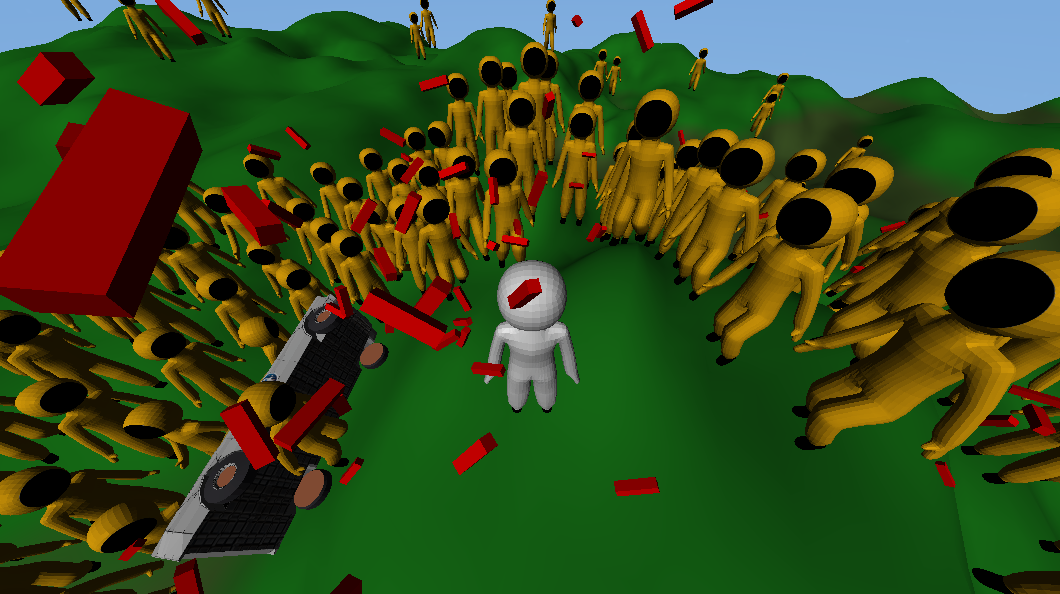
\includegraphics[width=0.8\textwidth]{chapters/results/sections/gameplay/resources/lots-of-stuff.png}
    \caption{BepuPhysics library taken to the extremee}
    \label{fig:bepu-lots-of-stuff}
\end{figure}